\clearpage
\section{Appendix}
\label{sec:appendix}
% \begin{itemize}
%     \item show RAG templates for all models 
% \end{itemize}

\label{sub:data-col-pre}
% \todo{@donghao: double check appendix}
\subsection{Data Collection and Preprocessing}
\label{sec:data}
% \todo{remove rapget}
We evaluate our proposed metric, \rap, using two tasks of question answering and machine translation. For question answering, we use \webqsp and \ms. The \textbf{\webqsp} dataset \cite{yih2016value} is a widely used benchmark for KBQA task. We selected a subset of 1008 questions from test data, mainly following the criteria as for WebQSP-WD \cite{C18-1280} that to keep questions with at least one acceptable answer in Wikidata. 
% , a subset of WebQSP containing only questions with at least one acceptable answer in Wikidata. We retrieved up to 10 documents per query from Wikipedia for the RAG-based question answering task.
\textbf{\ms} (Microsoft Machine Reading Comprehension) is a comprehensive dataset for reading comprehension and question answering, released by Microsoft\footnote{\url{https://microsoft.github.io/msmarco/}}. For our experiments, we used the dataset created by \cite{huang2024performance}. This dataset includes 100 queries, each with well-formed answers across five categories: LOCATION, NUMERIC, PERSON, DESCRIPTION, and ENTITY, totaling 500 queries. Each query is accompanied by 10 passages that provide context for the RAG-based question answering task.
For machine translation task, we use the \textbf{\mac} (Manually Aligned Chinese-English) dataset curated by \cite{huang2025optimizing}. This dataset comprises sentences from six Chinese novels and their corresponding English translations, spanning a diverse range of genres, including humor, martial arts, classics, war, romance, and science fiction. It contains a total of 5,661 entries, with 4,528 used for training and 1,133 reserved for testing.

\noindent
\textbf{Preparing Context-Data for \webqsp} 
\label{sub:webqsp}
To evaluate open-source LLMs using various prompting strategies, including Retrieval-Augmented Generation (RAG), we crawled Wikipedia for relevant documents to address \webqsp questions. We developed a Python script to prepare the context data by retrieving up to 10 documents per query, which were then processed through text extraction, segmentation, and embedding. These document chunk embeddings were stored locally for vector search. For each question, we retrieved the 8 most relevant document chunks through similarity search to form the context for RAG prompting.

% \begin{enumerate}
% \textbf{WebQSP}: Introduced by \cite{yih2016value}, the WebQuestionsSP (WebQSP) dataset is a widely used benchmark for knowledge-based question answering (KBQA) over structured data. For our experiments, we selected 1008 queries from the WebQSP-WD dataset \cite{C18-1280}, a subset of WebQSP containing only questions with at least one acceptable answer in Wikidata. We retrieved up to 10 documents per query from Wikipedia for the RAG-based question answering task.
% \textbf{MS MARCO}: MS MARCO (Microsoft Machine Reading Comprehension) is a comprehensive dataset for reading comprehension and question answering, released by Microsoft\footnote{\url{https://github.com/microsoft/MSMARCO-Question-Answering\#qa}}. For our experiments, we selected 100 queries with well-formed answers across five categories: LOCATION, NUMERIC, PERSON, DESCRIPTION, and ENTITY, resulting in a test dataset of 500 queries. Each query in the dataset is accompanied by 10 passages used as context for the RAG-based question answering task.
% \end{enumerate}
% The resulting datasets, WebQSP-RAPGeT and MS MARCO-RAPGeT, have very similar structures, each containing the following elements:
% \begin{enumerate}
%     \item \textbf{id}: retrieved from the source dataset
%     \item \textbf{question}: retrieved from the source dataset
%     \item \textbf{answers}: retrieved from the source dataset
%     \item \textbf{context}: for MS MARCO, the context is created by merging the passages from the source dataset. The method for creating contexts for WebQSP is detailed in Section \ref{sub:webqsp}.
% \end{enumerate}
% Regarding ground-truth answers, \ms includes an element called \textbf{wellFormedAnswers} retrieved from the source dataset, which serves as ground truth for performance evaluation using BLEU and Rouge-L scores. Whereas, \webqsp ground-truth answers contain lists of entities

% Additionally, MS MARCO-RAPGeT includes an element called \textbf{wellFormedAnswers} retrieved from the source dataset, which serves as ground truth for performance evaluation using BLEU and RougeL scores.
% 
% Unlike MS MARCO-RAPGeT, the WebQSP-RAPGeT dataset contains only gold entities in the answers element, which are used as ground truths. We developed a novel evaluation method, detailed in Section \ref{sec:gemini}, to assess the generated texts against these entity ground truths.

\noindent


% \subsection{Creation of Context for \webqsp}
% Since we want to evaluate open-source LLMs for different prompting strategies including RAG which requires providing relevant data to the question, we crawl documents from Wikipedia containing relevant information for answering questions in \webqsp. To create the context data element for the \webqsp dataset, we developed a Python script using LangChain\footnote{\url{https://github.com/langchain-ai/langchain}}, a framework designed to simplify the creation of applications using LLMs. The script first retrieved up to 10 documents per query from Wikipedia. These documents were then processed through text extraction, segmentation, and embedding procedures utilizing the LangChain framework and the HuggingFace Instructor text embedding model\footnote{\url{https://huggingface.co/hkunlp/instructor-large}}, resulting in the generation of embeddings. These embeddings, along with the source document chunks, were efficiently stored locally using FAISS\footnote{\url{https://ai.meta.com/tools/faiss}}, an open-source library for vector search created by Meta, which facilitates streamlined document retrieval. The script ran for more than 7 hours to complete processing all 1008 questions. Finally, for each question in the dataset, we used another script to retrieve the 8 most relevant document chunks through similarity search and combined them to form the context while performing RAG prompting.

% We aim to evaluate open-source LLMs for various prompting strategies, including RAG, which requires providing relevant data to the question. To conduct the experiments, we crawled documents from Wikipedia containing pertinent information for answering questions in the \webqsp. We developed a Python script using LangChain\footnote{\url{https://github.com/langchain-ai/langchain}}, a framework designed to simplify the creation of applications using LLMs, to prepare context data for \webqsp questions. 
% The script first retrieved up to 10 documents per query from Wikipedia. These documents were then processed through text extraction, segmentation, and embedding procedures using the LangChain framework and the HuggingFace Instructor text embedding model\footnote{\url{https://huggingface.co/hkunlp/instructor-large}}, resulting in the generation of embeddings. These embeddings, along with the source document chunks, were efficiently stored locally using FAISS\footnote{\url{https://ai.meta.com/tools/faiss}}, an open-source library for vector search created by Meta, which facilitates streamlined document retrieval. The script ran for over 7 hours to complete processing all 1008 questions. Finally, for each question in the dataset, we used another script to retrieve the 8 most relevant document chunks through similarity search and combined them to form the context while performing RAG prompting.

%Processing all 1008 questions took over 7 hours.

\subsection{LLM-based KBQA Evaluation} 
\label{sec:gemini}
% Why it is not straightforward to evaluate LLM's output for this. Because KBQA answers are list of entities, but output is freetext. Propose to use an independent LLM (Gemini) to assist in evaluating. 

\begin{listing}[t]
\begin{minted}[breaklines=true,fontsize=\small]{text}
You are evaluating a question answering task. The ground-truth answer is a list of answer-items. 
First, extract the answer-items from the generated answer. 
Then, map each generated answer-item to the ground-truth answer-item if possible. If no matching, use an empty list.
Output using the following format. {"predicted_answer": [list of answer-items extracted from the generated answer], "mappings": {"predicted_answer_1": [matched groundtruth answers], "predicted_answer_2": []}}

Question: <KBQA Question>
Ground-truth answer: <KBQA Ground-truth Answer>
Generated answer: <LLM-generated Answer>
\end{minted}
\caption{Prompt template for KBQA evaluation using Gemini Pro. The actual content will be filled in the placeholders of \textit{Question}, \textit{Ground-truth answer}, and \textit{Generated answer}. }
\label{list:gemini_prompt}
\end{listing}

\begin{figure}
    \centering
    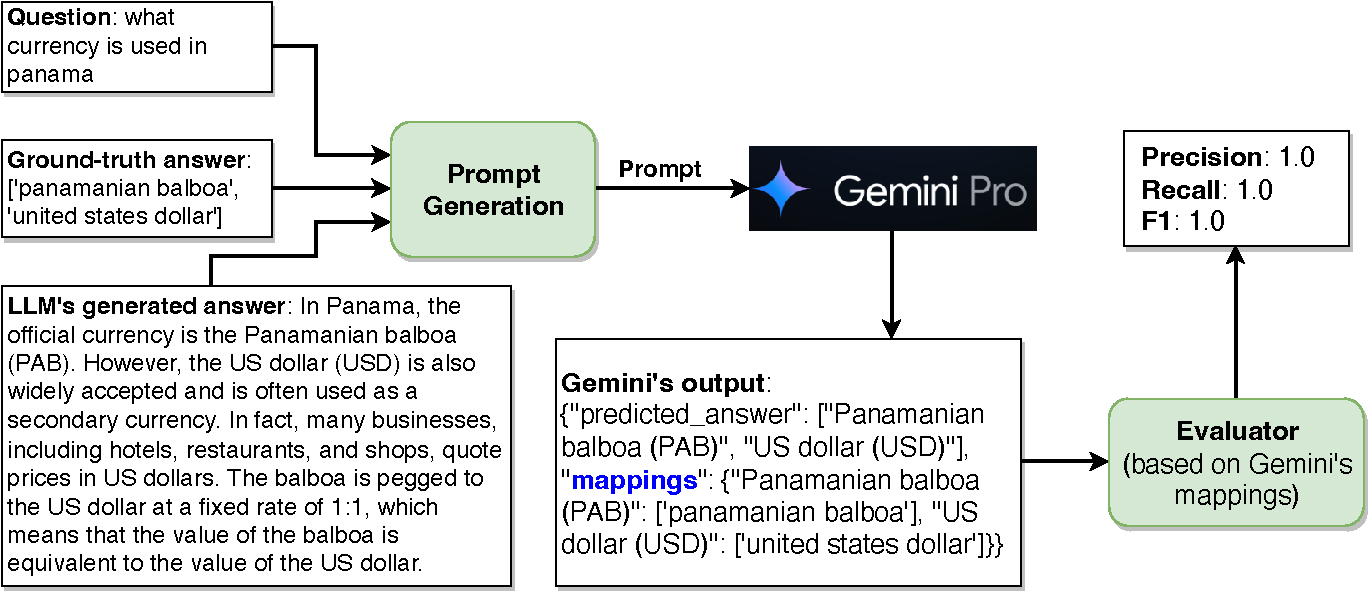
\includegraphics[width=.5\textwidth]{image/gemini_eval.pdf}
    \caption{LLM-based KBQA evaluation workflow using prompts for precision, recall, and F1 scores with Gemini-1.0-Pro as evaluator.}
    %\caption{LLM-based KBQA Evaluation Workflow. Given the input of \textit{question}, \textit{ground-truth answer}, and \textit{LLM's generated answer}, we create a prompt to extract answer-items and map them to ground-truth answer-items. Then, we calculate the precision, recall, and F1 based on the mappings of generated and ground-truth answer-items. We use Gemini-1.0-Pro for this evaluation task.} %The generated answer is taken from Llama 3-8B. }
    \label{fig:gemini_eval}
\end{figure}

% In KBQA task, the most common type of answer is a list of entities from the KG. For example, the answer to the question ``What language is spoken in Switzerland?'' is ``[Italian language, German language, French, Romansh language]''. While we can request LLMs to generate answers in the format of a list of entities, not all LLMs consistently follow this output format request. Therefore, it is crucial to process the answers returned by LLMs to extract the entity list for evaluation. One solution is to use Named Entity Recognition (NER); however, answers can contain other types of information besides named entities. Additionally, the wording used in answers might differ from the KG's entities even though they refer to the same entity, such as ``United States Dollar'' versus ``US dollar (USD)''.

% To resolve this problem, we propose an LLM-based evaluation method where an LLM is requested to extract answer-items (entities) from the generated answer and map them to the ground-truth answer-items. Figure \ref{fig:gemini_eval} shows the LLM-based KBQA evaluation workflow with an actual example using an answer generated from Llama 3-8B. We first construct a prompt using our pre-defined prompt template, shown in Listing \ref{list:gemini_prompt}. The prompt contains the input question, ground-truth answer, LLM's generated answer, and a request to extract answer-items and map them to the ground-truth answer-items. As shown in Figure \ref{fig:gemini_eval}, Gemini outputs a list of \textit{predicted answers} and a \textit{mapping} which maps each item in the predicted answers with those in ground-truth answers. Noted that one predicted answer-item can be mapped to more than one ground-truth answer-item or none (i.e., wrong answer). 

In the KBQA task, answers are typically lists of entities from the KG. For instance, the answer to ``What language is spoken in Switzerland?'' is ``[Italian, German, French, Romansh]''. While LLMs can be asked to generate entity lists, they do not always follow this format. Therefore, processing LLM-generated answers to extract entity lists for evaluation is crucial. Using Named Entity Recognition (NER) alone is not sufficient because answers may include non-entity information and differing entity wordings, e.g., ``United States Dollar'' versus ``US dollar (USD)''.
To address this, we propose an LLM-based evaluation method where an LLM extracts and maps answer-items (entities) from the generated answer to the ground-truth entities. Figure \ref{fig:gemini_eval} illustrates this workflow with an example generated by Llama-3-8B. We construct a prompt using a predefined template (Listing \ref{list:gemini_prompt}), including the question, ground-truth answer, LLM-generated answer, and a request for entity extraction and mapping. As shown in the figure, Gemini outputs a list of \textit{predicted answers} and a \textit{mapping} of predicted answers to ground-truth answers. A predicted answer can map to multiple ground-truth items or none (i.e., incorrect answer).

The mapping is then used to compute evaluation metrics including Precision, Recall, and F1. The details are as follows. 
Given a question, we denote the ground-truth answer as $A=[A_1, A_2, \cdots, A_n]$ and the list of predicted answer-items as $\hat{A}=[\hat{A}_1, \hat{A}_2,\cdots, \hat{A}_m]$. The mapping is denoted as $M=\{\hat{A}_1: M_1, \hat{A}_2: M_2, \cdots, \hat{A}_m: M_m\}$ where $M_i$ is a list of ground-truth answer-items matched with the corresponding predicted answer-item, i.e., $M_i \subseteq A$ ($i=1, \cdots, m$) and $M_i$ is empty when the predicted answer-item is wrong. A predicted answer-item is called \textit{correct} if it matches with at least one of the ground-truth answer-items.
We define $c_G=|\text{set}(M_1\cup M2 \cup \cdots \cup M_m)|$ as the number unique ground-truth answer-items that matched with at least one predicted answer-item and $c_P$ as the number of correct predicted answer-items. The final number of correct answers is chosen as the smallest number between $c_G$ and $c_P$. 
% :
% \begin{align}
%     c = \left\{\begin{matrix}
% c_G & \text{if } c_G < c_P\\ 
% c_P & \text{otherwise} 
% \end{matrix}\right.
% \end{align}
This is to deal with the cases where different predicted answer-items carry the same meaning (mapped to the same ground-truth answer-item). The precision and recall are then computed as $\frac{c}{|\hat{A}|}$ and $\frac{c}{|A|}$, respectively. 
% follows: 
% \begin{align}
%     \text{precision} = \frac{c}{|\hat{A}|}
% \end{align}
% \begin{align}
%     \text{recall} = \frac{c}{|A|}
% \end{align}
F1 score is computed as the harmonic mean of precision and recall. 
We chose \gemini for this evaluation task because of its strong natural language processing capabilities and its availability during our experiments.

\subsection{Tuning RPP for All Models and Datasets}
\label{sec:gain_all}
\begin{figure}[ht]
    \centering
    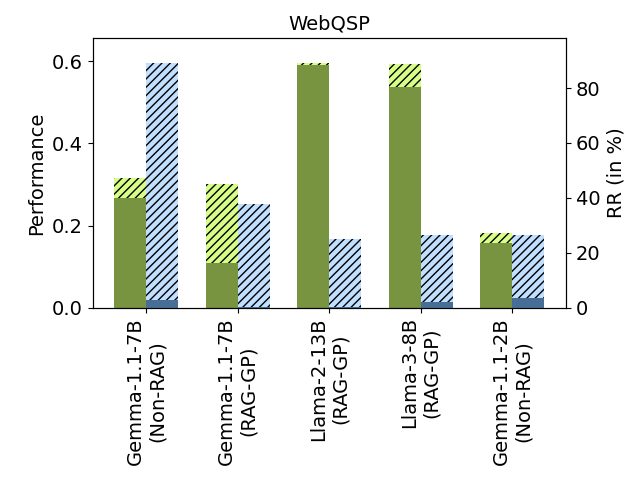
\includegraphics[width=1\linewidth]{image/chart_00_selected_wd.png}
    \caption{Top-5 model with highest RR reduction for \webqsp dataset}
    \label{fig:chart_00_selected_wd}
\end{figure}
\begin{figure}[ht]
    \centering
    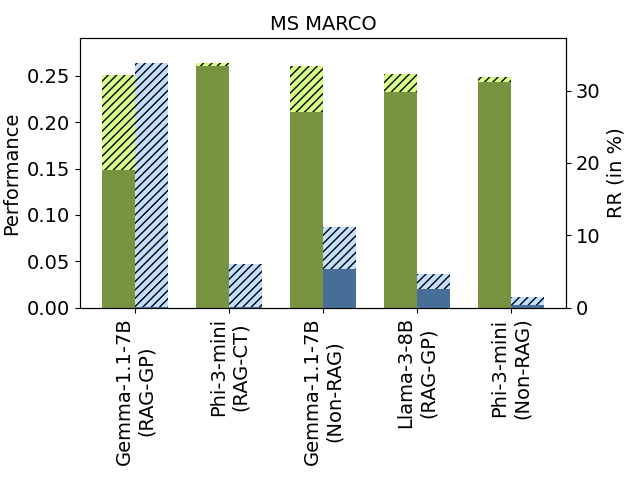
\includegraphics[width=1\linewidth]{image/chart_00_selected_mm.png}
    \caption{Top-5 model with highest RR reduction for \ms dataset}
    \label{fig:chart_00_selected_mm}
\end{figure}
\begin{figure}[ht]
    \centering
    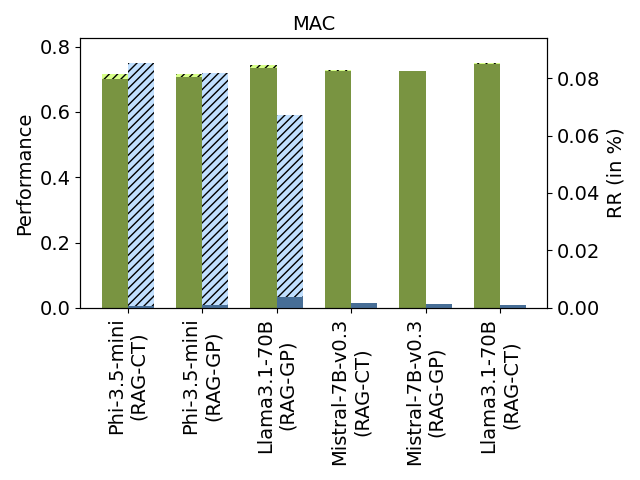
\includegraphics[width=1\linewidth]{image/chart_00_selected_mac.png}
    \caption{Tuning RPP of all models for \mac dataset}
    \label{fig:chart_00_selected_mac}
\end{figure}

We visualize the best performance when tuning RPP using original evaluation metrics (Original) and our proposed repetition-aware performance metric (RAP). RAP helps find RPP values that minimally reduce performance while significantly lowering repetition ratio (RR). Results for all models across three datasets are shown in Figure \ref{fig:chart_00_specific} (\webqsp, \ms) and \ref{fig:chart_00_selected_mac} (\mac). Figure \ref{fig:chart_00_selected_wd} and \ref{fig:chart_00_selected_mm} show the top-5 highest RR reduction after tuning for \webqsp and \ms dataset respectively. Green color bar indicates performance and blue color bar indicates RR. The hatched bar visualize the magnitude of reduction after tuning. 

\subsection{How Severe can Repetition be for Other Models and Datasets?}
\label{sec:how_severe}
Figure \ref{fig:webqsp_top3} visualize the top-3 highest and lowest RR for WebQSP, while Figure \ref{fig:chart_02_wd_all}, \ref{fig:chart_02_mm_all}, and \ref{fig:chart_02_mac_all} visualize all models for \webqsp, \ms, \mac respectively. The leftmost three models show the Top-3 highest RR, while the rightmost three display the lowest. The ratio of repeated text length to text length is also visualized. Colored squares above each point indicate the percentage of repeated questions, with blue, yellow, and red squares marking values below 10\%, between 10-20\%, and above 20\% respectively. The x-label indicates the model, the prompting method, and the RP of the RR. 
\begin{figure}[t]
    \centering
    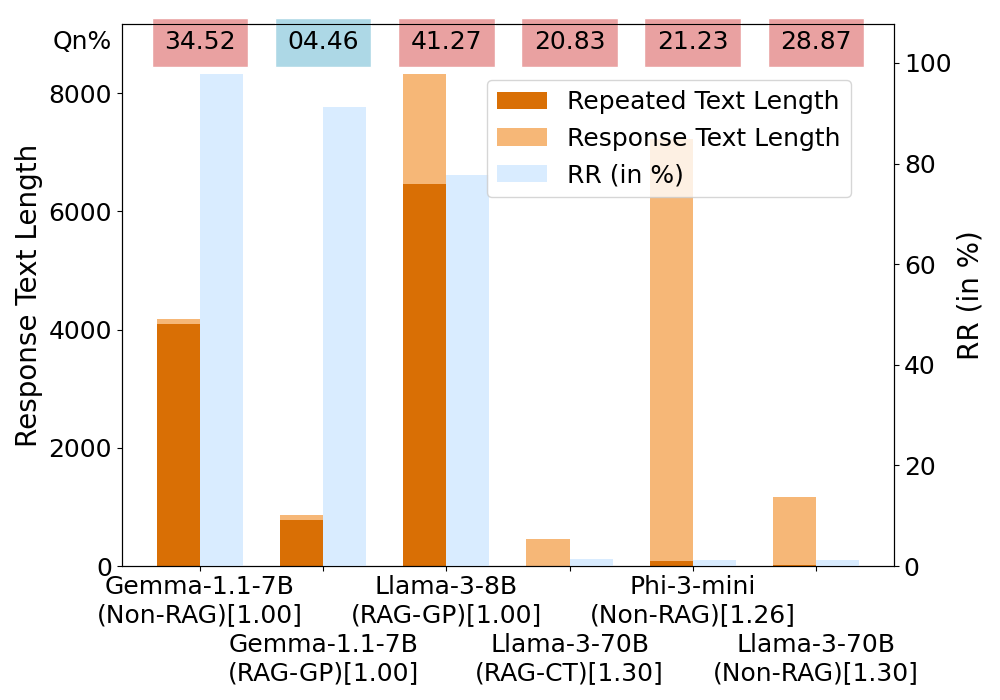
\includegraphics[width=1\linewidth]{image/chart_02_wd.png}
    \caption{Top-3 highest and lowest RR for \webqsp dataset}
    \label{fig:webqsp_top3}
\end{figure}
\begin{figure}[t]
    \centering
    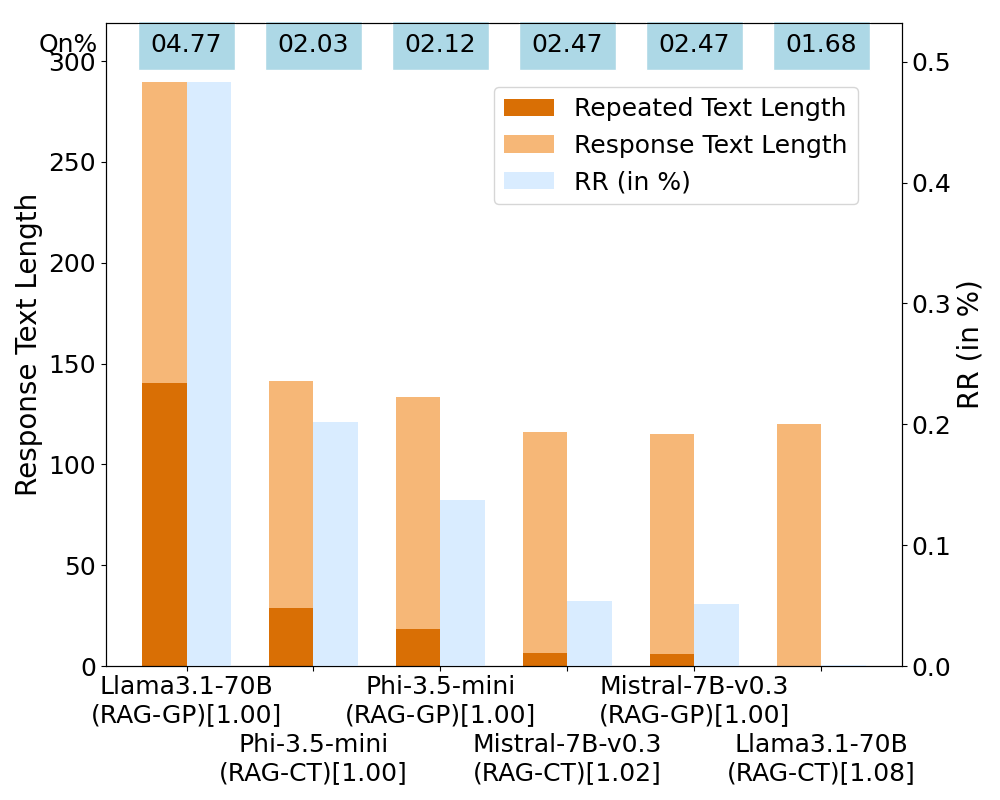
\includegraphics[width=1\linewidth]{image/chart_02_mac_all.png}
    \caption{Percentage of repeated responses, repeated text length, and RR for \mac dataset}
    \label{fig:chart_02_mac_all}
\end{figure}
\begin{figure*}[t]
    \centering
    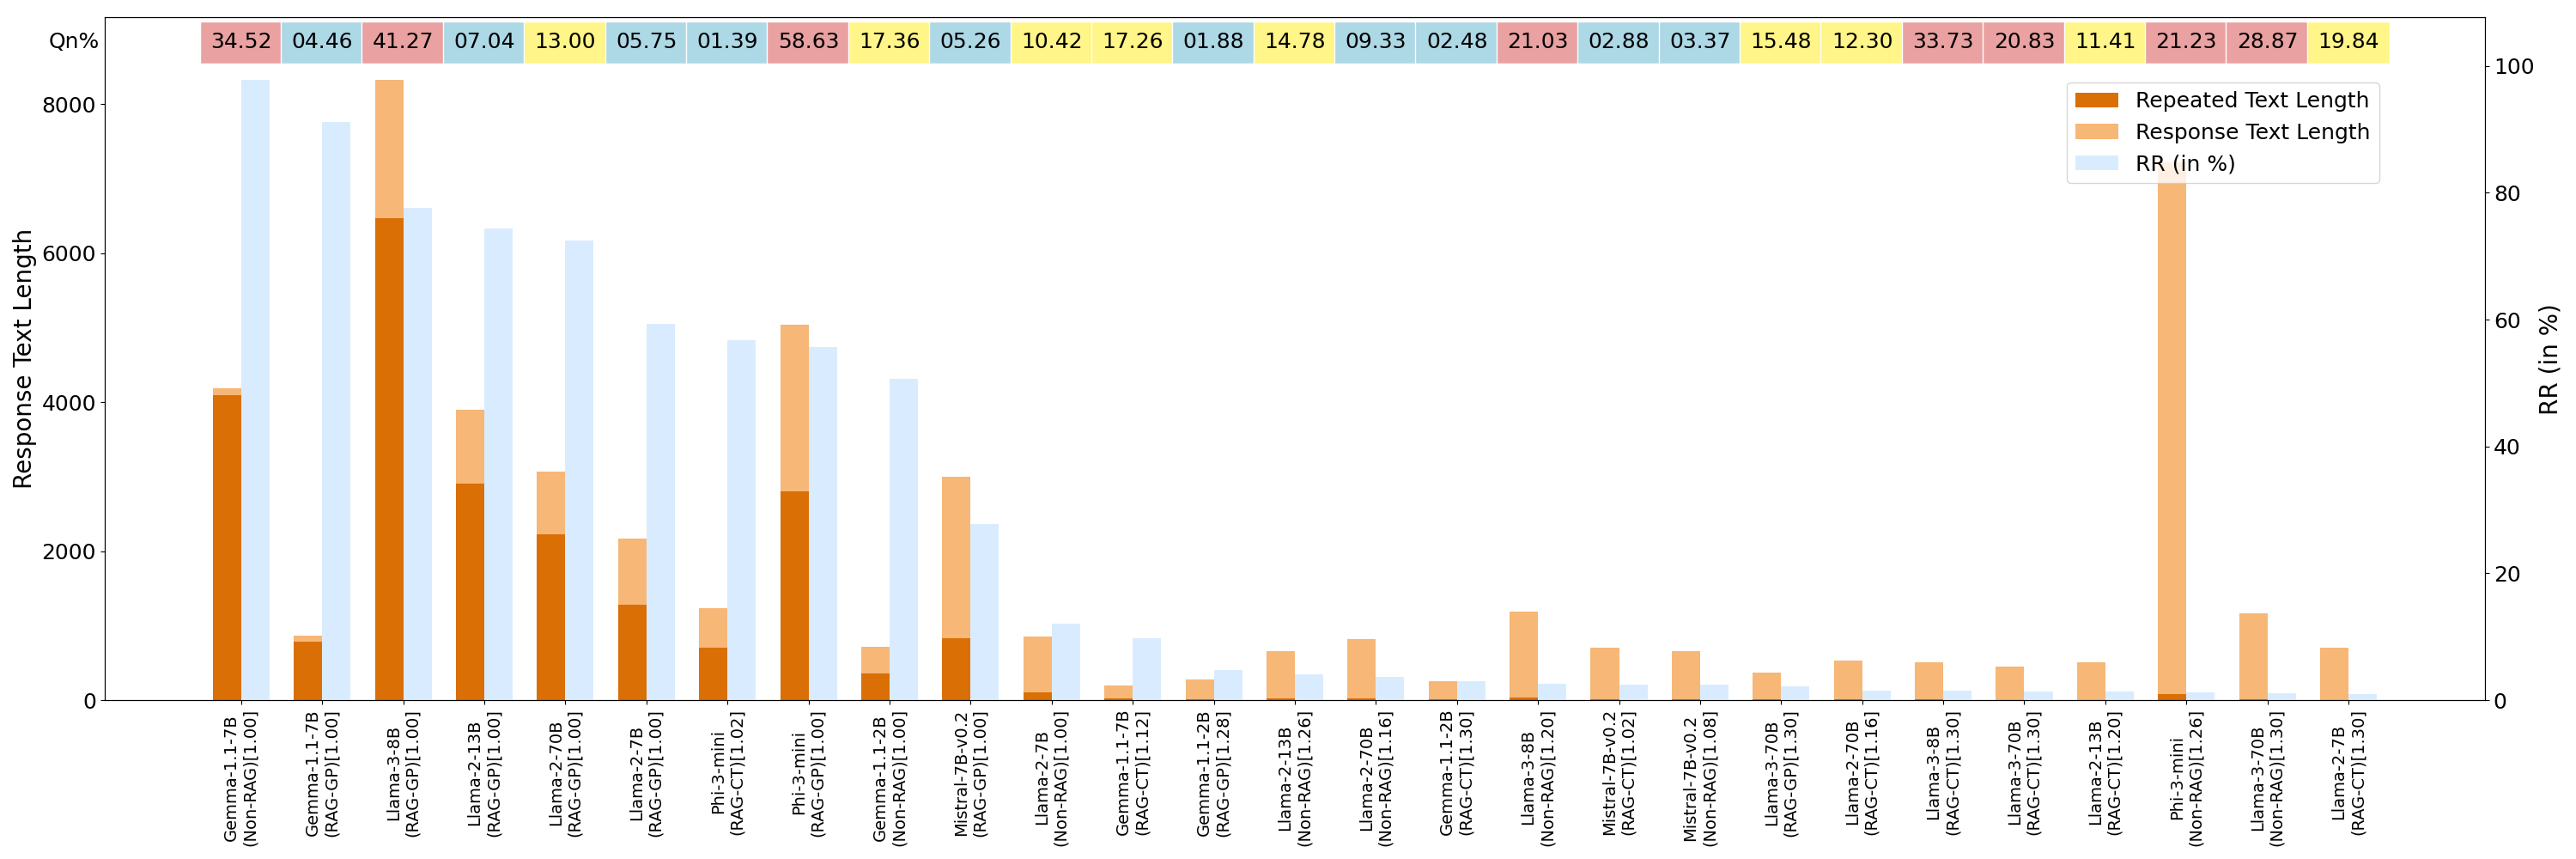
\includegraphics[width=\textwidth]{image/chart_02_wd_all.png}
    \caption{Percentage of repeated responses, repeated text length, and RR for \webqsp dataset}
    \label{fig:chart_02_wd_all}
\end{figure*}
\begin{figure*}[t]
    \centering
    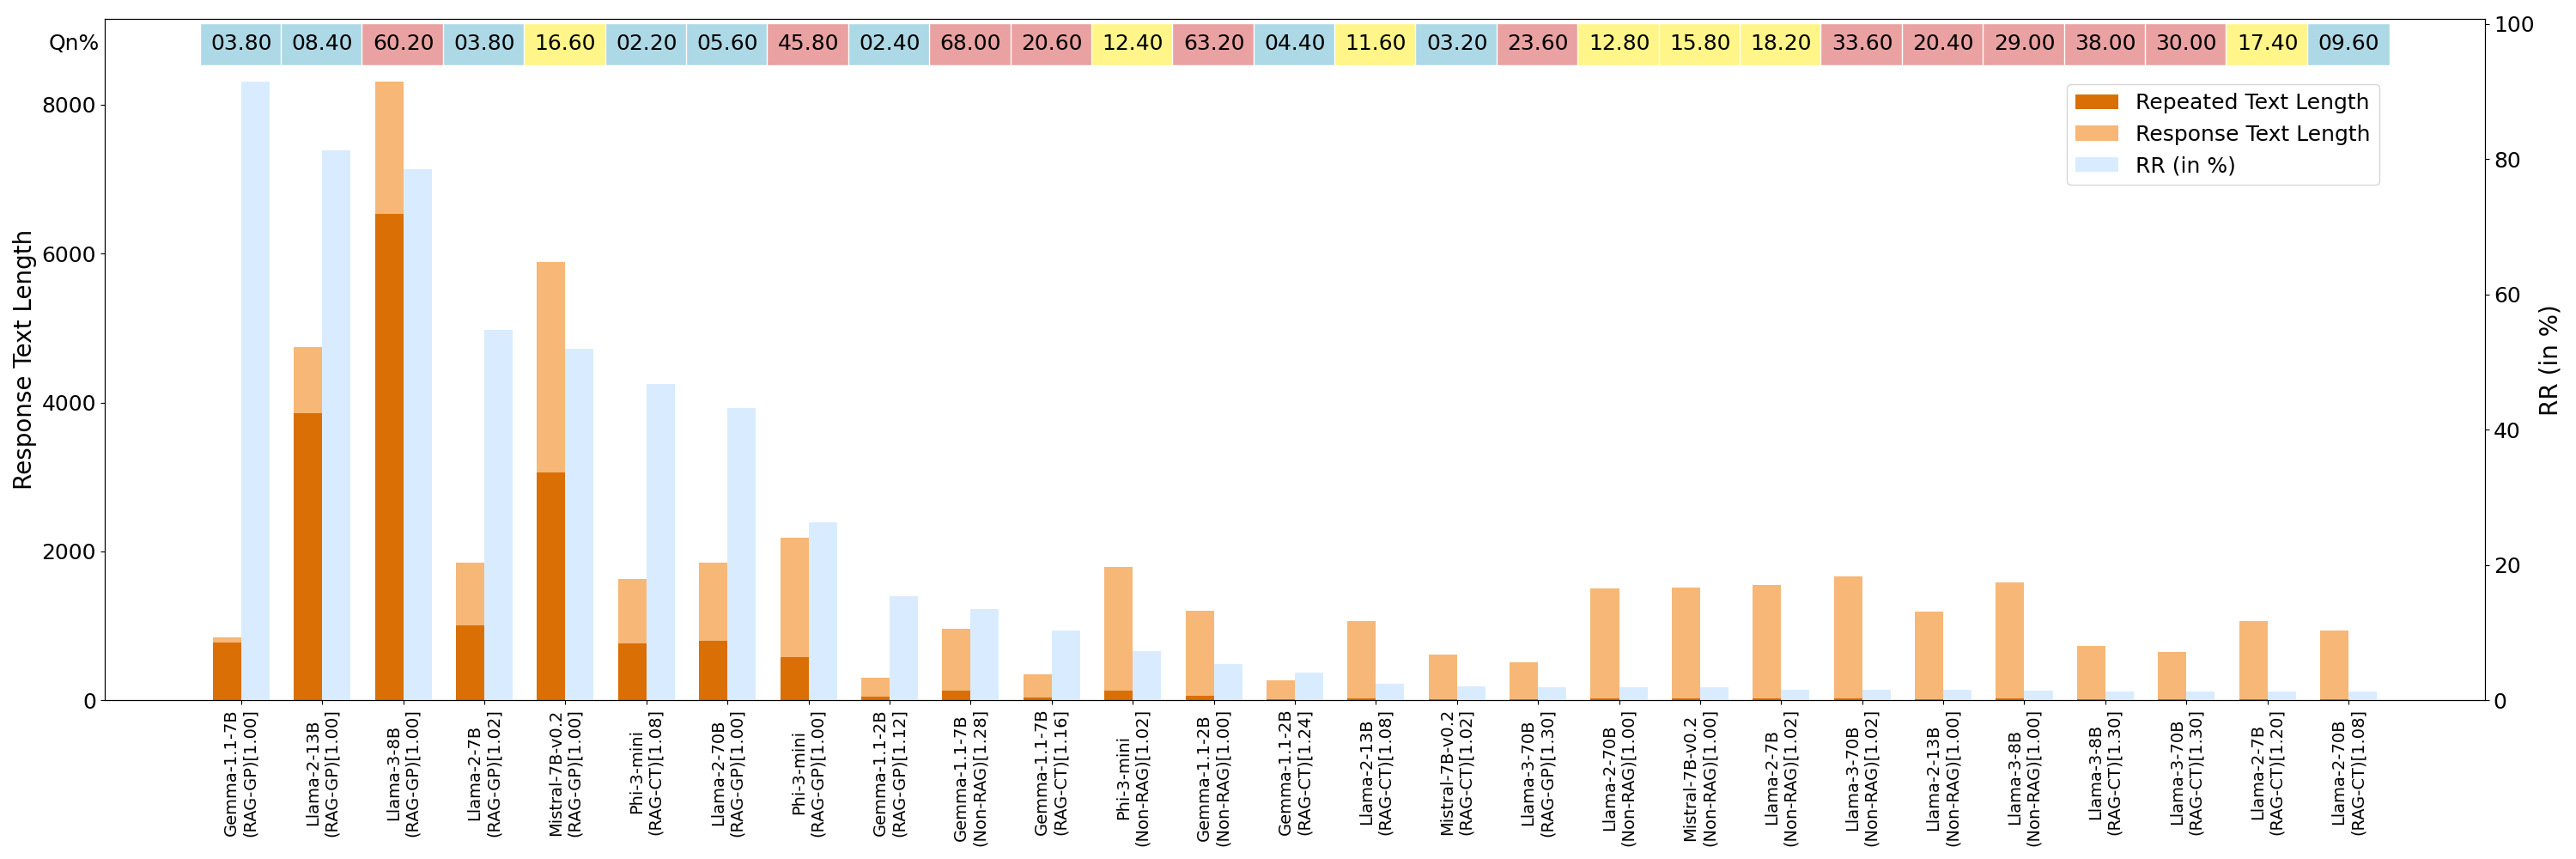
\includegraphics[width=\textwidth]{image/chart_02_mm_all.png}
    \caption{Percentage of repeated responses, repeated text length, and RR for \ms dataset}
    \label{fig:chart_02_mm_all}
\end{figure*}
\begin{figure*}[t]
    \centering
    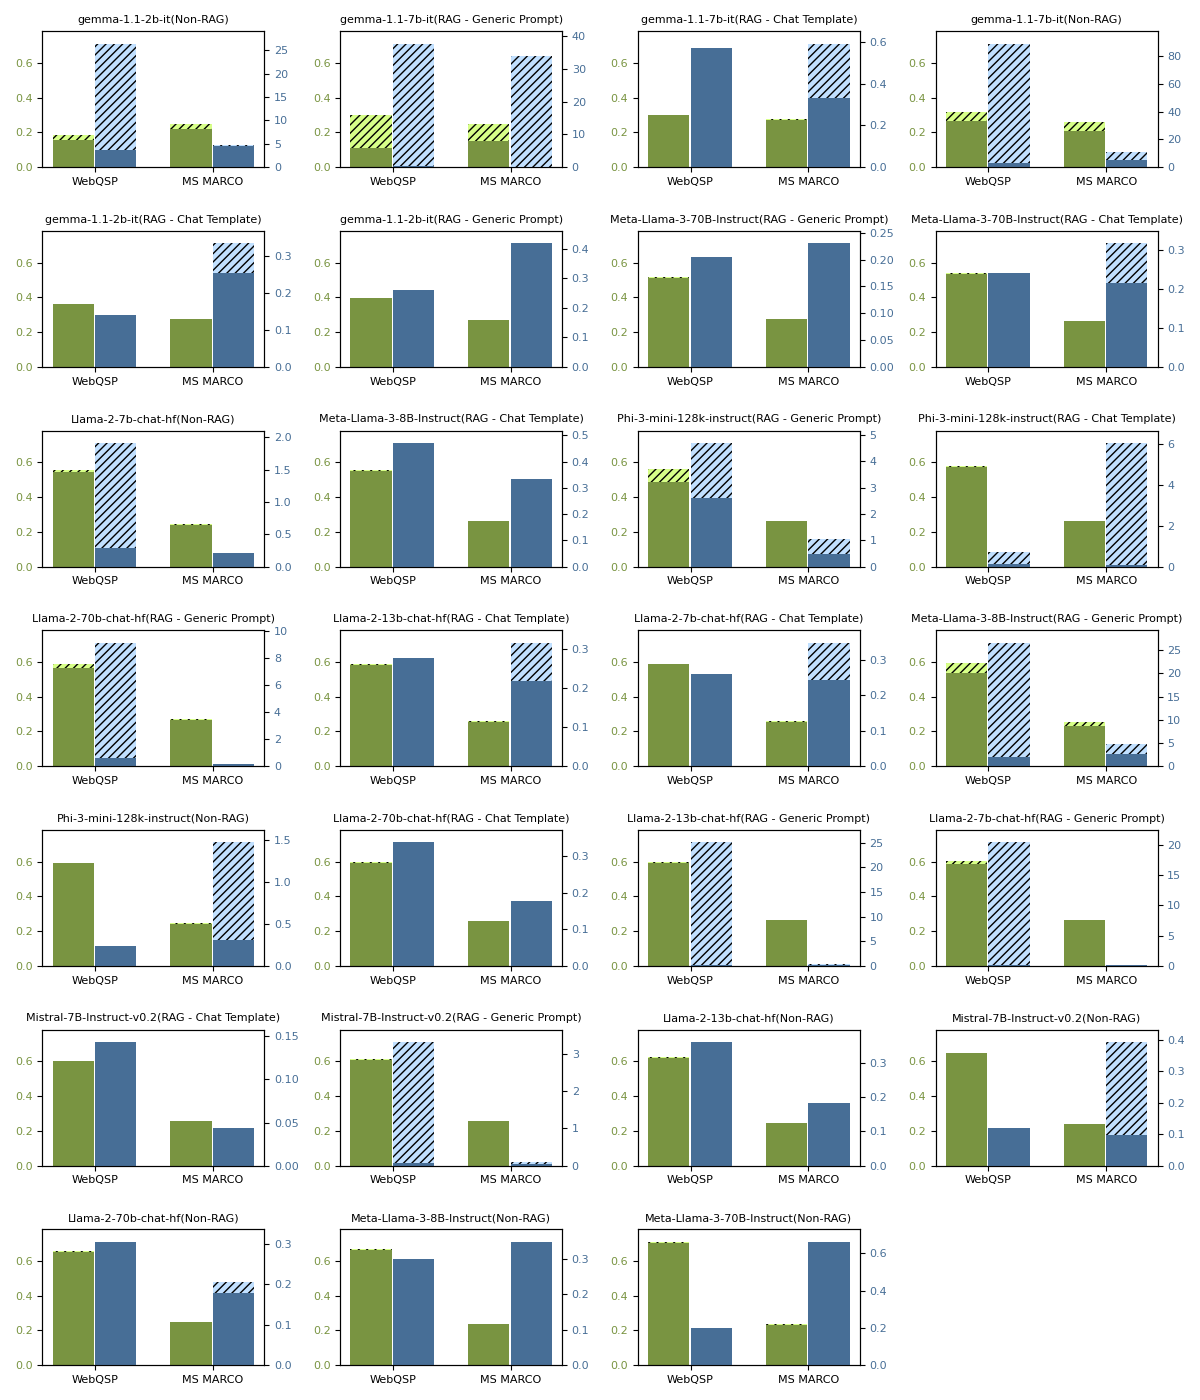
\includegraphics[width=\textwidth]{image/chart_00_specific.png}
    \caption{Tuning RPP of all models for \webqsp and \ms dataset}
    \label{fig:chart_00_specific}
\end{figure*}



\subsection{Evaluating the Quality of Gemini's Evaluation} 
\label{sec:eval_gemini}

To assess the effectiveness of our LLM-based KBQA evaluation method, we randomly selected 100 samples from the experiment results of the Llama-3-70B Non-RAG model, as this configuration achieved the best performance on WebQSP. A human evaluator was then asked to review and provide feedback on Gemini’s evaluation of these samples (following the process described earlier). The agreement rate between the human evaluator and Gemini was 89.0\%. While this indicates that the method is not flawless, it demonstrates a high level of reliability, making our LLM-based KBQA evaluation suitable for automatically assessing LLM responses in KBQA tasks.

\begin{table*}[]
\centering
\small
\resizebox{\textwidth}{!}{
\begin{tabular}{c|p{.1\textwidth}|p{.1\textwidth}|p{.4\textwidth}|p{.4\textwidth}}
\toprule
No. & Question                                     & Ground-truth               & LLM Response (Llama 3-70B)                                                                                                                                                                                                         & Gemini's Evaluation                                                                                                                                                                                                                                            \\ \midrule
1   & who is robin roberts father            & {[}lawrence e. roberts{]}                  & Robin Roberts father is Lawrence   E. Roberts, a pilot in the United States Air Force and a colonel. He passed   away in 2004.                                                                                       & \{\textbf{predicted\_answer}: {[}Lawrence E.   Roberts{]}, \textbf{mappings}: \{Lawrence E. Roberts: {[}lawrence e. roberts{]}\}\}                                                                                                                                           \\\midrule
2   & who does michael oher play for in 2010 & {[}baltimore ravens{]}                     & In 2010, Michael Oher played for   the Baltimore Ravens.                                                                                                                                                             & \{\textbf{predicted\_answer}: {[}Baltimore   Ravens{]}, \textbf{mappings}: \{Baltimore Ravens: {[}baltimore ravens{]}\}\}                                                                                                                                                    \\\midrule
3   & who was queen   elizabeth ii mom       & {[}'queen elizabeth the queen   mother'{]} & Queen Elizabeth II's mother was   Queen Elizabeth The Queen Mother, also known as Elizabeth Bowes-Lyon. She was   the wife of King George VI and the mother of Queen Elizabeth II and Princess   Margaret.           & \{"\textbf{predicted\_answer}":   {[}"Queen Elizabeth The Queen Mother", "Elizabeth   Bowes-Lyon"{]}, "\textbf{mappings}": \{"Queen Elizabeth The Queen   Mother": {[}'queen elizabeth the queen mother'{]}, "Elizabeth   Bowes-Lyon": {[}{]}\}\}                            \\\midrule
4   & where was rihanna born and raised      & {[}saint michael parish{]}                 & Rihanna was born in Saint   Michael, Barbados, and raised in Bridgetown, Barbados.                                                                                                                                   & \{\textbf{predicted\_answer}: {[}Saint   Michael, Bridgetown{]}, \textbf{mappings}: \{Saint Michael: {[}saint michael parish{]},   Bridgetown: {[}{]}\}\}                                                                                                                    \\\midrule
5   & what country was king tut s tomb found & {[}egypt{]}                                & King Tuts tomb, also known as   KV62, was discovered in Egypt. Specifically, it was found in the Valley of   the Kings, a necropolis in Luxor, Egypt, on November 4, 1922, by British   archaeologist Howard Carter. & \{\textbf{predicted\_answer}: {[}Egypt,   Valley of the Kings, Luxor, Egypt, November 4, 1922, Howard Carter{]},   \textbf{mappings}: \{Egypt: {[}egypt{]}, Valley of the Kings: {[}{]}, Luxor: {[}{]}, Egypt: {[}{]},   November 4, 1922: {[}{]}, Howard Carter: {[}{]}\}\} \\\bottomrule
\end{tabular}}
% \caption{Using \gemini for KBQA evaluation: It correctly maps answer-items in most cases, though occasional inaccuracies occur. Human-Gemini agreement is high (89.0\%) in Llama 3-70B, Non-RAG setting.}
\caption{Showing example of using \gemini for evaluating KBQA task. In many cases, Gemini can extract predicted answer-items and generate the mappings correctly, but sometimes it failed to extract the correct prediction, making the evaluation inaccurate. Nevertheless, a human evaluation of 100 samples showed a high agreement between human and Gemini of 89.0\%. LLM Response is taken from Llama 3-70B, Non-RAG setting.}
\label{tab:gemini-eval}
\end{table*}

We conducted a qualitative analysis of the proposed LLM-based KBQA evaluation using \gemini (Section \ref{sec:gemini}). Table \ref{tab:gemini-eval} presents examples of outputs from Llama-3-70B for five WebQSP questions, along with the corresponding evaluations from Gemini. 

In the first example, Gemini correctly extracts the answer item "Lawrence E. Roberts" and accurately maps the predicted answer to the ground-truth answer, resulting in a precise evaluation. A similar correct evaluation occurs in the second example.

However, Gemini occasionally fails to extract the correct information from the generated text. In the third question, for example, Gemini mistakenly identifies "Elizabeth Bowes-Lyon" as part of the predicted answer, despite the LLM response not implying this. This error leads to a precision score of only 0.5 for this answer, negatively affecting the LLM's overall performance evaluation. A similar issue occurs in the fifth question, where Gemini extracts too many keywords from the LLM response, yielding a very low final score, despite the fact that the predicted answer is correct when reading the response in context.

In summary, to further evaluate the quality of our LLM-based KBQA evaluation method, we randomly selected 100 samples from the Llama-3-70B Non-RAG model’s results, as this configuration performed the best on WebQSP. A human evaluator reviewed Gemini's assessments, and the agreement rate was 89.0\%. While not perfect, this indicates that our LLM-based KBQA evaluation method demonstrates a strong level of reliability and can be effectively utilized for automatically evaluating LLM responses in KBQA tasks.

\iffalse
\subsection{Overview of Large Language Models}
\label{subsec:overview_llms}

This study evaluates a diverse set of open-source large language models (LLMs) across question answering (QA) and machine translation (MT) tasks. For QA tasks, we assess nine models:

\begin{itemize}
    \item Llama-2 series (7B, 13B, 70B parameters)
    \item Llama-3 series (8B, 70B parameters)
    \item Gemma-1.1 series (2B, 7B parameters)
    \item Phi-3-mini (3.8B parameters)
    \item Mistral-7B
\end{itemize}

For the MT task, we evaluate three models:

\begin{itemize}
    \item Phi-3.5-mini (3.8B parameters)
    \item Mistral-7B
    \item Llama-3.1-70B
\end{itemize}

Table~\ref{tab:ai_models} provides a comprehensive overview of these models, detailing their respective companies, model names, HuggingFace model identifiers, and the tasks for which they were evaluated. This selection encompasses a wide range of parameter sizes and architectures, representing the current state-of-the-art in open-source LLM development.

This diverse selection allows for a robust comparison across different model families and sizes, providing insights into the relative strengths of various open-source LLMs in both QA and MT tasks.

\begin{table}[htbp]
\caption{Overview of Large Language Models and Their Specifications by Task}
\label{tab:ai_models}
\centering
\resizebox{\columnwidth}{!}{
\begin{tabular}{l|l|l|l}
\toprule
\textbf{Company} & \textbf{Model Name} & \textbf{HuggingFace Model ID} & \textbf{Task} \\
\midrule
\multirow{6}{*}{Meta} & Llama-2-7B & meta-llama/Llama-2-7b-chat & QA \\
& Llama-2-13B & meta-llama/Llama-2-13b-chat & QA \\
& Llama-2-70B & meta-llama/Llama-2-70b-chat & QA \\
& Llama-3-8B & meta-llama/Meta-Llama-3-8B-Instruct & QA \\
& Llama-3-70B & meta-llama/Meta-Llama-3-70B-Instruct & QA \\
& Llama-3.1-70B & shenzhi-wang/Llama3.1-70B-Chinese-Chat & MT \\
\midrule
\multirow{2}{*}{Microsoft} & Phi-3-mini & microsoft/Phi-3-mini-128k-instruct & QA \\
& Phi-3.5-mini & microsoft/Phi-3.5-mini-instruct & MT \\
\midrule
\multirow{2}{*}{Google} & Gemma-1.1-2B & google/gemma-1.1-2b-it & QA \\
& Gemma-1.1-7B & google/gemma-1.1-7b-it & QA \\
\midrule
\multirow{2}{*}{Mistral AI} & Mistral-7B-v0.2 & mistralai/Mistral-7B-Instruct-v0.2 & QA \\
& Mistral-7B-v0.3 & shenzhi-wang/Mistral-7B-v0.3-Chinese-Chat & MT \\
\bottomrule
\end{tabular}
}
\end{table}
\fi


\subsection{Prompt Templates}
\label{sec:prompt}
In this section, we present the various prompt templates used for different tasks and configurations in our experiments. These templates guide the interaction between the models and the provided input, ensuring consistency across models and tasks. The templates cover both question answering (QA) and machine translation (MT) tasks, with specialized designs for models with and without retrieval-augmented generation (RAG) capabilities. Each template is structured with placeholders that dynamically incorporate the question, context, or input data. The following listings describe the prompt templates in detail.

\begin{listing}[H]
\begin{minted}[breaklines=true,fontsize=\small]{text}
Use the following pieces of context to answer the question at the end. If you don't know the answer, just say that you don't know, don't try to make up an answer.
{context}
Question: {question}
Helpful Answer:
\end{minted}
\caption{RAG - Generic Prompt template for question answering. The placeholders \textit{\{question\}} and \textit{\{context\}} will be filled with the question and the retrieved data, respectively.}
\label{list:rag-generic}
\end{listing}

\begin{listing}[H]
\begin{minted}[breaklines=true,fontsize=\small]{text}
<|begin_of_text|>
<|start_header_id|>
system
<|end_header_id|>
You are a chatbot having a conversation with a human.
<|eot_id|>
<|start_header_id|>user
<|end_header_id|>
{question}
<|eot_id|>
<|start_header_id|>
Assistant
<|end_header_id|>
\end{minted}
\caption{Non-RAG prompt template for question answering with Llama-3 models. The placeholder \textit{\{question\}} will be filled with the question.}
\label{list:non-rag}
\end{listing}

\begin{listing}[H]
\begin{minted}[breaklines=true,fontsize=\small]{text}
<|begin_of_text|>
<|start_header_id|>
system
<|end_header_id|>
You are a chatbot having a conversation with a human.
<|eot_id|>
<|start_header_id|>user
<|end_header_id|>
Use the following pieces of context to answer the question at the end. If you don't know the answer, just say that you don't know, don't try to make up an answer.
{context}
Question: {question}
<|eot_id|>
<|start_header_id|>
Assistant
<|end_header_id|>
\end{minted}
\caption{RAG - Chat Template for Llama-3 models. The placeholders \textit{\{question\}} and \textit{\{context\}} will be filled with the question and retrieved data, respectively.}
\label{list:rag-chat}
\end{listing}

\begin{listing}[H]
\begin{minted}[breaklines=true,fontsize=\small]{text}
You will be given a Chinese sentence to translate. If it is an incomplete sentence, or if you are unsure about the meaning, simply copy the input text as your output. Do not output any additional sentences, such as explanations or reasoning.
Chinese: {input}
\end{minted}
\caption{Machine Translation - Generic Prompt (\mtgen) for all models. The placeholder \textit{\{input\}} will be filled with the Chinese sentence retrieved from the \mac testing set.}
\label{list:mt-generic}
\end{listing}

\begin{listing}[H]
\begin{minted}[breaklines=true,fontsize=\small]{text}
<|begin_of_text|>
<|start_header_id|>
system
<|end_header_id|>
You are a helpful assistant that translates Chinese to English.
<|eot_id|>
<|start_header_id|>user
<|end_header_id|>
You will be given a Chinese sentence to translate. If it is an incomplete sentence, or if you are unsure about the meaning, simply copy the input text as your output. Do not output any additional sentences, such as explanations or reasoning.
Chinese: {input}
<|eot_id|>
<|start_header_id|>
Assistant
<|end_header_id|>
\end{minted}
\caption{Machine Translation - Chat Template (\mttem) for Llama-3 models. The placeholder \textit{\{input\}} will be filled with the Chinese sentence retrieved from the \mac testing set.}
\label{list:mt-chat}
\end{listing}